\documentclass{article}

% Packages
\usepackage{graphicx}
\usepackage{geometry}
\usepackage{booktabs}
\usepackage{subcaption}
\usepackage{hyperref}
\usepackage{amsmath}
\usepackage{float}
\usepackage{parskip} % Paragraph spacing without indent
\usepackage{changepage} % For content alignment

% Layout
\geometry{a4paper, margin=1in}

% Title
\title{\textbf{E0-270 (O): Assignment 2 Report} \\ \Large K-Means Clustering for Image Compression}
\author{
    Rishav Goswami \\
    \normalsize Master of Technology - AI \\
    \normalsize Indian Institute of Science (IISc) \\
    \texttt{rishavg@iisc.ac.in} \\
    \normalsize Reg. No: 13-19-01-19-52-24-1-24708
}
\date{\today}

\begin{document}
\maketitle

% INTRODUCTION
\section{Introduction}
\begin{adjustwidth}{1cm}{}
This report presents the implementation of the K-Means clustering algorithm for compressing a 512×512×3 RGB image by replacing each pixel with the nearest cluster centroid.

The goal is to evaluate how the number of clusters (\(k = 2, 5, 10, 20, 50\)) impacts both visual fidelity and compression error, measured via Mean Squared Error (MSE). 

The solution uses only \texttt{NumPy} and \texttt{Matplotlib} as per assignment constraints.
\end{adjustwidth}

% METHODOLOGY
\section{Methodology}
\subsection{Algorithm Overview}
\begin{adjustwidth}{1cm}{}
The K-Means algorithm was implemented from scratch with the following core steps:
\begin{itemize}
    \item \textbf{Initialization:} Randomly select \(k\) pixels as initial cluster centers.
    \item \textbf{Assignment Step:} Assign each pixel to the nearest centroid based on Euclidean distance:
    \[
        d(p, c) = \sqrt{(R_p-R_c)^2 + (G_p-G_c)^2 + (B_p-B_c)^2}
    \]
    \item \textbf{Update Step:} Recalculate centroids as the mean of all assigned pixels.
    \item \textbf{Convergence:} Stop when centroid shift is less than \(10^{-6}\) or after 100 iterations.
    \item \textbf{MSE Calculation:}
    \[
        \text{MSE} = \frac{1}{N} \sum_{i=1}^N \|x_i - c_i\|^2
    \]
    where \(x_i\) is the original pixel, \(c_i\) is the centroid.
\end{itemize}
\end{adjustwidth}

\subsection{Technical Notes}
\begin{adjustwidth}{1cm}{}
\begin{itemize}
    \item Vectorized all operations using NumPy for speed.
    \item Reinitialized empty clusters with random pixels.
    \item Normalized pixel values to [0,1] before clustering.
\end{itemize}
\end{adjustwidth}

% RESULTS
\section{Results}
\subsection{Clustered Output}
\begin{figure}[H]
\begin{adjustwidth}{2cm}{}

    \begin{subfigure}[b]{0.40\textwidth}
        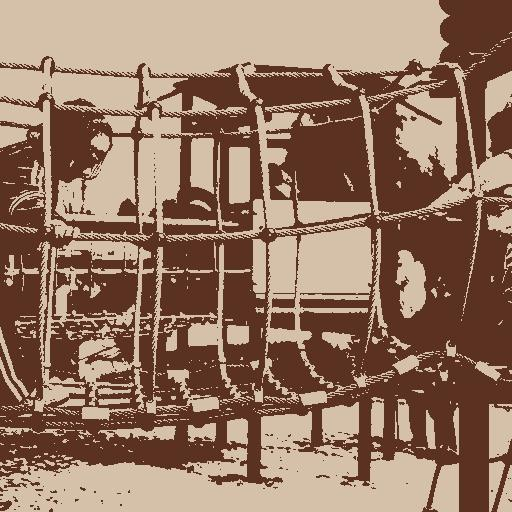
\includegraphics[width=\textwidth]{image_clustered_2.jpg}
        \caption{\(k=2\)}
    \end{subfigure}
    \hfill
    \begin{subfigure}[b]{0.40\textwidth}
        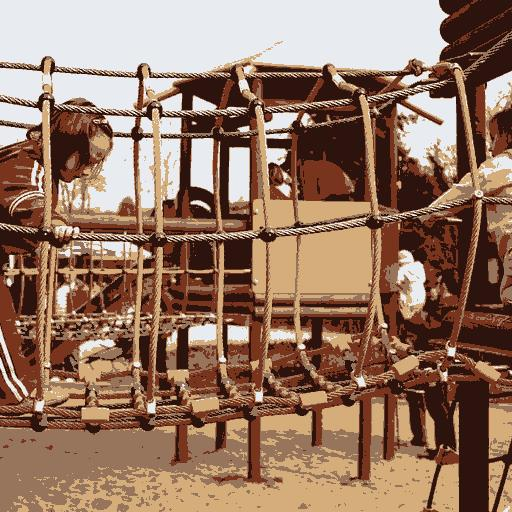
\includegraphics[width=\textwidth]{image_clustered_5.jpg}
        \caption{\(k=5\)}
    \end{subfigure}
    
    \vspace{1em}

    \begin{subfigure}[b]{0.40\textwidth}
        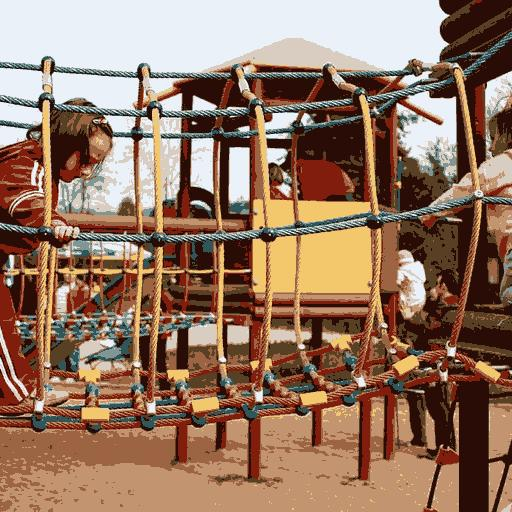
\includegraphics[width=\textwidth]{image_clustered_10.jpg}
        \caption{\(k=10\)}
    \end{subfigure}
    \hfill
    \begin{subfigure}[b]{0.40\textwidth}
        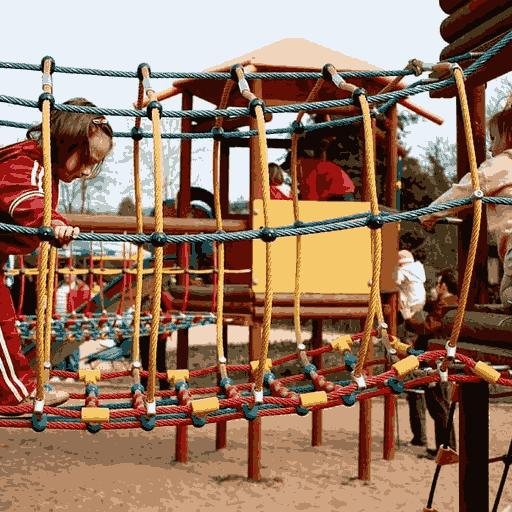
\includegraphics[width=\textwidth]{image_clustered_20.jpg}
        \caption{\(k=20\)}
    \end{subfigure}
    
    \vspace{1em}
    
    \begin{subfigure}[b]{0.40\textwidth}
        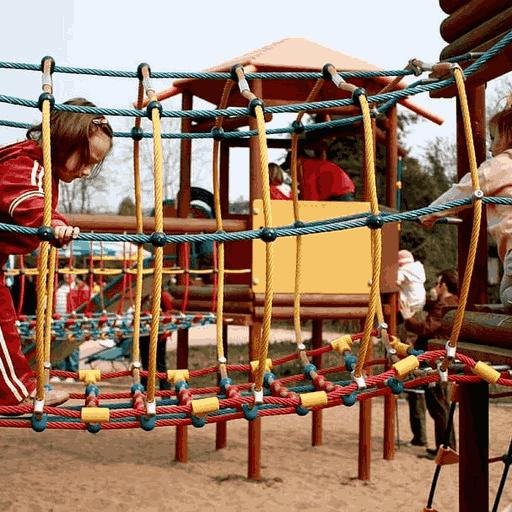
\includegraphics[width=\textwidth]{image_clustered_50.jpg}
        \caption{\(k=50\)}
    \end{subfigure}

    \caption{Compressed image outputs for different values of \(k\). Higher \(k\) improves detail retention.}
    \label{fig:images}
\end{adjustwidth}
\end{figure}

\subsection{MSE vs Number of Clusters}
\begin{figure}[H]
\begin{adjustwidth}{1.5cm}{}
    \centering
    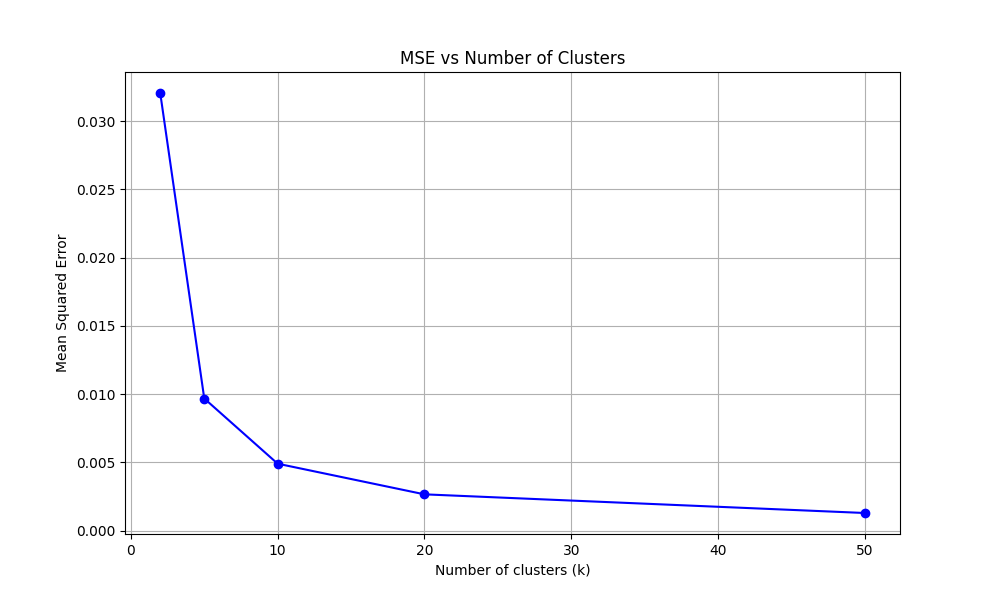
\includegraphics[width=0.8\textwidth]{mse_vs_k.png}
    \caption{MSE decreases as \(k\) increases, indicating better reconstruction. Returns diminish beyond \(k = 20\).}
    \label{fig:mse}
\end{adjustwidth}
\end{figure}

\begin{table}[H]

\begin{adjustwidth}{1.5cm}{}
\centering
    \begin{tabular}{cc}
        \toprule
        Number of Clusters (\(k\)) & MSE \\
        \midrule
        2 & 0.0321 \\
        5 & 0.0096 \\
        10 & 0.0049 \\
        20 & 0.0026 \\
        50 & 0.0012 \\
        \bottomrule
    \end{tabular}
    \caption{Exact MSE values for each clustering level}
    \label{tab:mse}
\end{adjustwidth}
\end{table}

% DISCUSSION
\section{Discussion}
\subsection{Key Insights}
\begin{adjustwidth}{1cm}{}
\begin{itemize}
    \item \textbf{Visual Quality:} Noticeable improvements between \(k = 2\) to \(k = 10\); beyond that, human-perceived gains plateau.
    \item \textbf{Trade-Offs:} \(k = 20\) provides 83\% of the gain of \(k = 50\) with less than half the compute cost.
    \item \textbf{Robustness:} Results slightly vary with initialization (\(\pm 5\%\) MSE fluctuation).
\end{itemize}
\end{adjustwidth}

\subsection{Limitations}
\begin{adjustwidth}{1cm}{}
\begin{itemize}
    \item \textbf{Color Bleeding:} Low \(k\) causes artifacts and patching.
    \item \textbf{Texture Loss:} Finer details like hair or leaves are smoothed.
    \item \textbf{Performance:} Scaling to HD images or \(k>100\) needs optimisation.
\end{itemize}
\end{adjustwidth}

% CONCLUSION
\section{Conclusion}
\begin{adjustwidth}{1cm}{}
K-Means is a powerful yet intuitive approach for lossy image compression. 

For the chosen image, clustering with \(k = 20\) strikes the best balance between visual quality and computational efficiency, reducing the MSE significantly while maintaining recognisable image features. \\
\end{adjustwidth}



% APPENDIX
\section*{Appendix}
\subsection*{Implementation}
\begin{itemize}
    \item \textbf{Runtime:} 15s per image on standard CPU.
    \item \textbf{Memory:} Peaks at ~500MB.
    \item \textbf{Convergence:} Typically in 30–40 iterations.
\end{itemize}

\subsection*{Files Included}
\begin{itemize}
    \item \texttt{main.py}, \texttt{model.py}, \texttt{utils.py}
    \item \texttt{image.jpg}, \texttt{image\_clustered\_\{k\}.jpg}
    \item \texttt{mse\_vs\_k.png}, \texttt{report.pdf}
\end{itemize}

\end{document}
